\documentclass{beamer}

\usepackage[T1]{fontenc}
\usepackage[spanish]{babel}
\usepackage{parskip}

\usepackage{hyperref}
\usepackage{graphicx}
\usepackage{float}

\title[Máster en Ingeniería Industrial]{Aplicación de técnicas de mejora continua en el Centro de Salud de Laguna de Duero}
\subtitle[]{Trabajo Fin de Máster}
\author{Luis Llamas Fernández}
\institute[]{Máster en Ingeniería Industrial}
\date{\today}

\begin{document}

\frame{\titlepage}

\begin{frame}{Índice}
    \tableofcontents[hideallsubsections]
\end{frame}

\AtBeginSection[ ]
{
    \begin{frame}{Índice}
        \tableofcontents[currentsection]
    \end{frame}
}

% Presentation structure
\section{Introducción}

\begin{frame}{Contexto y motivación}
    \begin{figure}
        \centering
        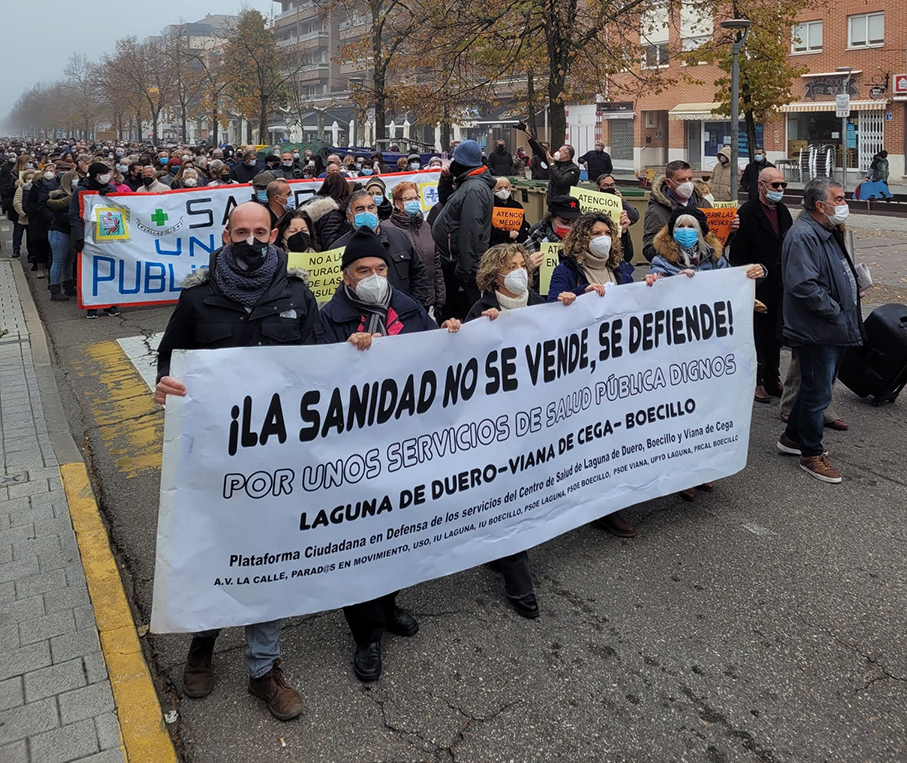
\includegraphics[height=0.7\textheight]{img/manifestacion.jpeg}
        \caption{Manifestación por la sanidad pública en Laguna de Duero}
    \end{figure}
\end{frame}

\begin{frame}{Objetivos}

    \begin{block}{Objetivo principal}
        Crear un \alert{estándar} por tipo de proceso de todas las tareas administrativas de la sección administrativa.
    \end{block}

    Con los siguientes \textbf{subobjetivos},

    \begin{enumerate}
        \item Crear un grupo de trabajo
        \item Crear lista de tareas estandarizadas por proceso
        \item Encontrar problemas más importantes
        \item Proponer mejoras respecto a los problemas encontrados
    \end{enumerate}
\end{frame}

\begin{frame}{Alcance}

\end{frame}

\section{Atención Primaria}

\begin{frame}{Cartera de servicios}
    
\end{frame}

\begin{frame}{Centro de Salud de Laguna de Duero}
    \begin{figure}
        \centering
        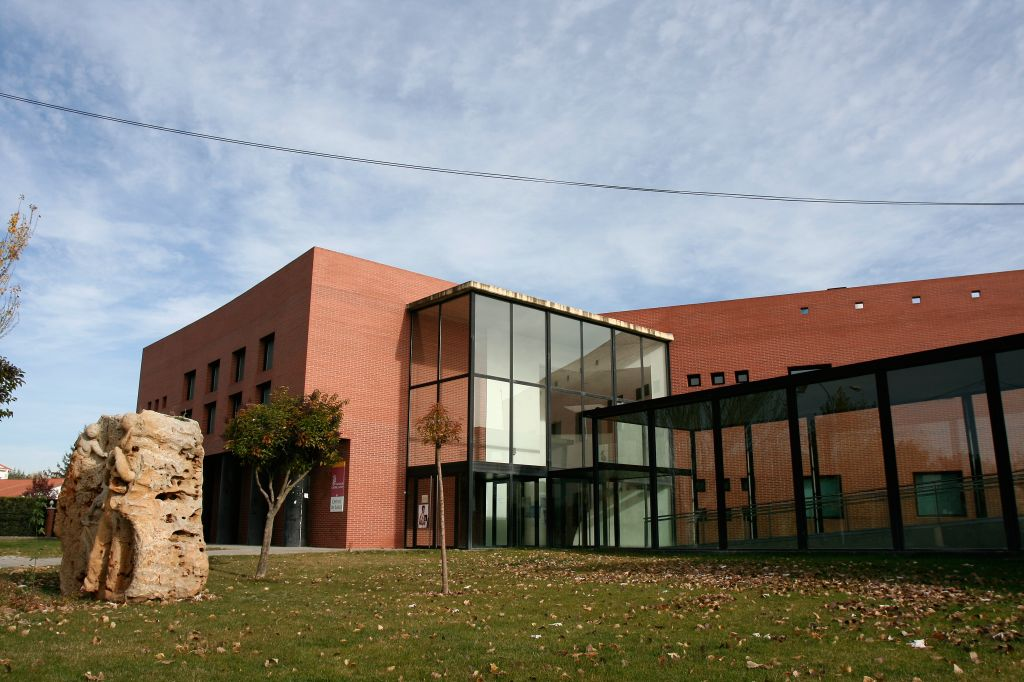
\includegraphics[height=0.7\textheight]{img/centro-salud.jpg}
        \caption{Fachada del Centro de Salud de Laguna de Duero}
    \end{figure}
\end{frame}

\section{Metodología}
\section{Desarrollo}
\subsection{Grupo de trabajo}
\subsection{Procesos}
\subsection{Análisis de las causas raíz}
\section{Conclusiones}

\end{document}